\documentclass{article}
\usepackage[utf8]{inputenc}
\usepackage{fullpage}
\usepackage[russian]{babel}
\usepackage{amssymb}
\usepackage{listings}
\usepackage{xcolor}
\usepackage{hyperref}
\usepackage{amsthm,amsmath,amsfonts,amssymb}
\usepackage{graphicx}

\lstset{
    language=Python,
    commentstyle=\color{gray!80!white}
}
\hypersetup{
    colorlinks=true,
    urlcolor=blue
}

\newcommand{\ProbSimple}[1]{\mathbf{#1}}
\newcommand{\ProbSign}[3]{\underset{#2}{\ProbSimple{#1}}\left[\;#3\;\right]}
\renewcommand{\Pr}[2]{\ProbSign{Pr}{#1}{#2}}
\newcommand{\Prw}[1]{\Pr{}{#1}}
\newcommand{\Ex}[2]{\ProbSign{E}{#1}{#2}}
\newcommand{\Exw}[1]{\Ex{}{#1}}
\newcommand{\Dp}[2]{\ProbSign{D}{#1}{#2}}
\newcommand{\Dpw}[1]{\Dp{}{#1}}
\newcommand{\F}{\mathbb{F}}
\newcommand{\Prr}{\ProbSimple{Pr}}

\title{Задачи по курсу ``Алгоритмы обработки потоковых данных''}
\date{Осень, 2014}

\begin{document}

\begin{center}
    {\Large Зачёт по курсу ``Алгоритмы обработки потоковых данных''}
    \vspace{0.3cm}

    {\large Казань, 2016}
\end{center}
\begin{flushright}
\textbf{oparin.vsevolod [at] gmail [dot] com}.\par
\href{https://docs.google.com/spreadsheets/d/1nsGop7vZAkOX1byVKugRFOMmGEu0Wg-MGzFm-ZxLfxo/edit?usp=sharing}{Таблица для зачета}\par
\end{flushright}

Для зачета нужно набрать 15 баллов (из 17 возможных). Набирать баллы можно следующим образом.
\begin{itemize}
    \item (1 балл) Решить один пункт одной задачи.
    \item (4 балла) Записать конспект лекции.
    \item (6 баллов) Написать визуализатор алгоритма.
\end{itemize}

\paragraph{Решение задачи.} Решения по каждой задаче пишите подробно. Настолько подробно, чтобы ваш одногруппник мог без ваших подсказок его понять. 

Все решения и вопросы присылайте на мой e-mail. В теме письма напишите ``Казань. Поточные алгоритмы. 2016. <Имя Фамилия>''. Крайне желательно оформлять решения в \LaTeX. Для простоты входа, я выкладываю исходник этого документа и шаблон на \href{https://github.com/vsevolod-oparin/streaming.2016-latex}{GitHub}.

\paragraph{Конспект лекции.} Перед тем, как писать конспект лекции, согласуйте это со мной. Я буду поддерживать в таблице с домашним заданием, кто какую лекцию взял. После того, как вы пришлете мне черновик, я могу попросить вас что-то исправить или добавить. Как только все исправления будут внесены, коспект засчитывается.

Конспект принимается только в \LaTeX.

\paragraph{Визуализатор.} Наиболее творческая часть зачета. Напишите визуализатор одного из алгоритмов. Я могу предложить вам написать такой для Count-Min скетча или Count скетча. Вы можете предложить свой. Для вдохновления посмотрите ссылки: \href{http://content.research.neustar.biz/blog/pcsa.html}{раз}, \href{http://content.research.neustar.biz/blog/hll.html}{два}, \href{http://content.research.neustar.biz/blog/runs.html}{три}. 

Хочется, чтобы визуализатор был доступен широким массам. Я предлагаю его реализовать на JavaScript, потом я его куда-нибудь выложу и прикреплю ссылку к описанию курса. Если есть идеи как сделать лучше, буду рад услышать.

Я представляю визуализатор примерно так:
\begin{center}
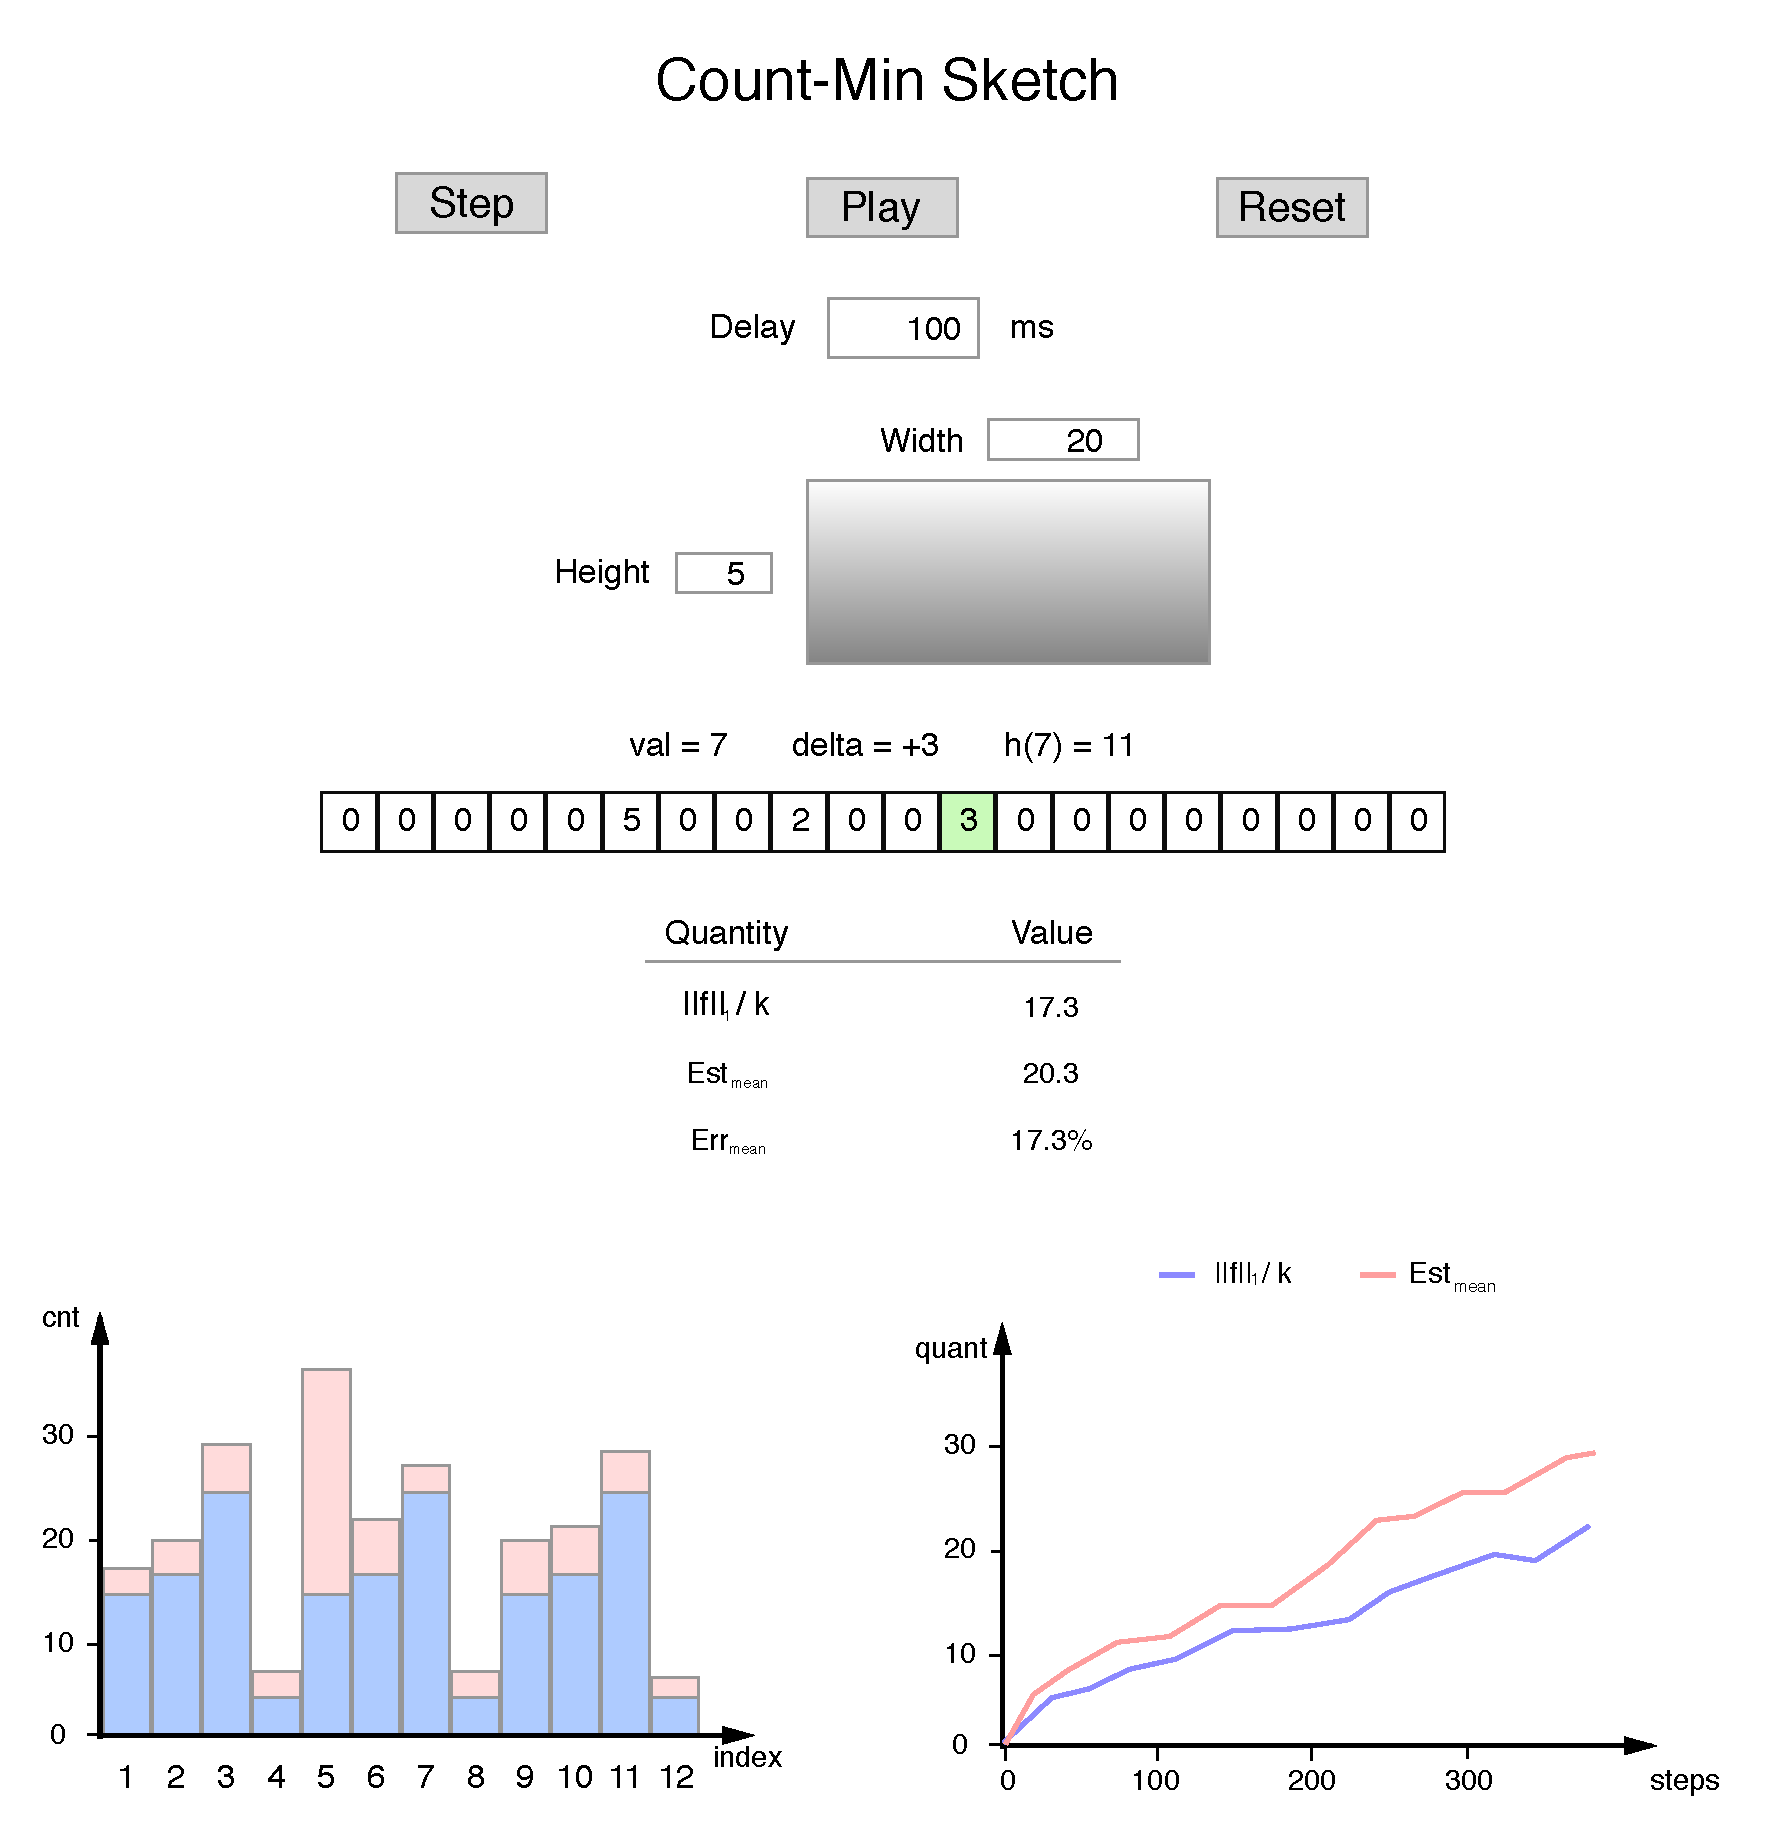
\includegraphics[scale=0.25]{cms.pdf}
\end{center}


\pagebreak
% \maketitle
\begin{center}
    {\large Теоретические задачи}
\end{center}

Для простоты, считайте что длина потока $m$ и размер множества $n$~-- величины одного порядка, т.е. $n = \Theta(m)$.

\paragraph{Задачи на последовательностях}
\begin{enumerate}

    \item Дана последовательность различных объектов $\sigma = \langle a_1, a_2, \cdots, a_m \rangle$, $a_i \in [n]$. Изначально длина последовательности неизвестна. Требуется за один проход выбрать 
    случайно подмножество из $k$ \textit{различных} объектов, используя $O(k \log n)$ памяти. Гарантируется, что $k \geq n$.

    \item Дана последовательность различных элементов $\sigma = \langle a_1, a_2, \cdots, a_m \rangle$, где $a_i \in [n]$. Требуется найти $k$-ую порядковую статистику: элемент последовательности, который встанет на $k$-ую позицию после сортировки. Разрешается выдать ответ с погрешностью $\varepsilon \cdot m$, т.е. вернуть такой элемент, чья позиция в отсортированной последовательности лежит в отрезке $[k - \varepsilon \cdot m, k + \varepsilon \cdot m]$. Решите задачу с вероятностью успеха $1 - \delta$, используя $O(\varepsilon^{-2} \cdot \log{\delta^{-1}} \log n)$.

    Что делать, если $m$ заранее неизвестно?

    \item Из набора чисел от $1$ до $n$ удалили все числа от $l$ до $r$, оставшиеся перемешали. Найдите за один проход $l$ и $r$. Память: $O(\log n)$.
        
    \item Дана последовательность элементов $\sigma = \langle a_1, \cdots, a_m \rangle$, $a_i \in [n]$. 
    В последовательности сушествует ровно два элемента, которые встречаются 1 раз. Остальные встречаются четное число раз. 
    \begin{enumerate}
        \item Найдите оба элемента детерминированно за $O(\log^2 n)$.
        \item Найдите оба элемента за $O(\log \delta^{-1} \log n)$ с вероятностью успеха $1 - \delta$. 
        \item Обобщите вероятностное решение для поиска $k$ уникальных элементов за $O(k^2 \log n)$ с вероятностью успеха $\geq \frac{1}{2}$.
        \item Оптимизируйте память до $O(k \log^2 (k \delta^{-1}) \log n)$ при условии, что алгоритм работает с вероятностью успеха $\geq 1 - \delta$.
    \end{enumerate}

\end{enumerate}

\paragraph{Задачи на графах}
\begin{enumerate}
    \setcounter{enumi}{4}
    \item Дан связный ориентированный граф в виде последовательности ребер на $n$ вершинах. Известно, что граф содержит Эйлеров путь, т.е. путь проходящий по всем ребрам ровно один раз. Эйлеров путь в ориентированном графе идет всегда по направлению ребра.
    \begin{enumerate}
        \item Найти начало и конец пути за один проход, детерминированно. Память $O(\log n)$.
        \item Пусть из стартовой вершины пути исходит ровно одно ребро. Докажите, что для поиска второй вершины пути детерминированный алгоритм использует $\Omega(n)$ памяти.
    \end{enumerate}

    \item Дан неориентированный граф на $n$ вершинах, содержащий Эйлеров путь. Постройте алгоритм, который находит за один проход оба конца Эйлерова пути c вероятностью $1 - \delta$. Память $O(\log \delta^{-1} \log n)$.
\end{enumerate}

\pagebreak

\paragraph{Нижние оценки}
$$
\begin{array}{|c|c|c|c|c|}
\hline
                & D^\rightarrow & R^{\rightarrow}_{\frac{1}{3}} & D & R_{\frac{1}{3}} \\
\hline 
\text{INDEX} & \geq n & \geq n & \leq \lceil \log n \rceil & \leq \lceil \log n \rceil \\
\text{EQ} & \geq n & O(\log n) & \geq n & O(\log n) \\
\text{DISJ} & \Omega(n) & \Omega(n) & \Omega(n) & \Omega(n) \\ \hline
\end{array}
$$

\begin{enumerate}
    \setcounter{enumi}{6}
 
    \item Дана последовательность $\sigma = \langle a_1, \cdots, a_m \rangle$, $a_i \in [n]$. Каждый элемент $x \in [n]$ присутствует в последовательности не более одного раза. Докажите, что точный детерминированный алгоритм, находящий наименьшее число $x \not\in \sigma$, использует $\Omega(n)$ памяти.

    \item Дана последовательность уникальных чисел $\sigma = \langle a_1, \cdots, a_m \rangle$, $a_i \in [n]$. Инверсия последовательности -- это пара индексов $i < j$ таких, что $a_i > a_j$. Четность последовательности -- это четность числа инверсий. Докажите, что однопроходный детерминированный алгоритм, определяющий четность, использует $\Omega(n)$ памяти.

    \item Докажите, что однопроходный алгоритм, который считает момент $F_2$ точно, использует $\Omega(n)$ памяти. Алгоритм может использовать случайные биты. Покажите, что если алгоритм использует $p$ проходов, ему потребуется хотя бы $\Omega(n / p)$ памяти.

    \item Покажите, что точный вероятностны однопроходный алгоритм для поиска медианы использует $\Omega(n)$ памяти.

    \item Есть невзвешенный неориентированный граф $G$, данный в виде потока ребер. Граф построен на $n$ вершинах. Требуется определить, есть ли в графе треугольник (три вершины, соединенные ребрами). Покажите, что однопроходный вероятностный алгоритм для этой задачи использует $\Omega(n^2)$ памяти.
\end{enumerate}

\paragraph{Хэш-функции}
\begin{enumerate}
    \setcounter{enumi}{11}

    \item Построим семейство хэш-функций $\mathcal{H} = \{h_i : \{0, 1\}^n \rightarrow \{0, 1\}^k\}_i$. 
    Функции хэшируют битовые строки длины $n$ в строки длины $k$ следующим образом. Берем случайно равновероятно битовую матрицу $A \in \{0, 1\}^{n \times k}$ и вектор $b \in \{0, 1\}^k$. Определим хэш-функцию 
    $$
    h_{A, b}(x) = A \cdot x + b^T,
    $$
    где все вычисления берутся по модулю 2. Докажите, что семейство хэш-функций 2-независимо.

    \item Пусть есть семейство функций $\mathcal{H} = \{h_i : K \rightarrow V\}_i$. Каждая функция семейства инъективна, т.е. любых различных $k_1, k_2 \in K$ выполняется $h_i(k_1) \neq h_i(k_2)$.
    Пусть известно, что для любого множества $A \subseteq K$ и любого ключа $k \in A$ выполняется равенство:

    $$
        \Pr{h_i \leftarrow U(\mathcal{H})}{h(k) = \min_{a \in A} h(a)} = \frac{1}{|A|}.
    $$

    Покажите, что для любых двух множеств $A, B \subseteq K$ выполняется условие:
    $$
        \Pr{h_i \leftarrow U(\mathcal{H})}{\min_{b \in B} h(b) = \min_{a \in A} h(a)} = \frac{|A \cap B|}{|A \cup B|}.
    $$
        
\end{enumerate}


\end{document}